\section{La croissance du f\oe tus (8 points)}

Lors de la grossesse d'une femme, les médecins surveillent à l'aide de l'échographie, les médecins surveillent la croissance du f\oe tus durant les 39 semaines de grossesse.

Voici quelques indicateurs de cette surveillance :
\begin{itemize}
	\item Durant les premières semaines, on mesure la longueur du f\oe tus (longueur tête-fesses).
	\item Ensuite, lorsque le f\oe tus est trop grand pour être visualisé complètement sur l'écran et donc être mesuré, on s'intéresse à la dimension de sa tête. On mesure le diamètre bipariétal (l'écartement entre les deux os qui se trouvent de chaque coté de la face, au dessus des oreilles). Le graphique ci-dessous donne le diamètre bipariétal d'une f\oe tus entre les semaines 11 à 24.
	
	\begin{center}
		\includegraphics[scale=0.2]{graph_foetus}
	\end{center}

\end{itemize}


\begin{questions}
	\question[2] 
		\begin{parts}
			\part[1] Déterminer graphiquement le diamètre bipariétal au bout de 11 semaines.
			\begin{solution}
				Le diamètre bipariétal à 11 semaines est d'environ 25 mm.
			\end{solution}
			
			\part[1] On désigne par $u_{11}$, $u_{12}$, ..., $u_{24}$ les valeurs du diamètre bipariétal pour les semaines 11 à 24. Quelle semble être la nature de la suite formée par ces termes successifs ?
			\begin{solution}
				Les points représentant les termes de la suite sont alignés, donc la suite est arithmétique.
			\end{solution}
		\end{parts}
	
	\question[2]
		Dans cette question, on étudie la croissance du f\oe tus durant les semaines 4 à 10. Dans un tableur, on saisit les données concernant la taille du f\oe tus et on fait calculer le rapport entre deux valeurs consécutives.
		Les résultats sont donnés dans le tableau suivant :
		
		\begin{center}
			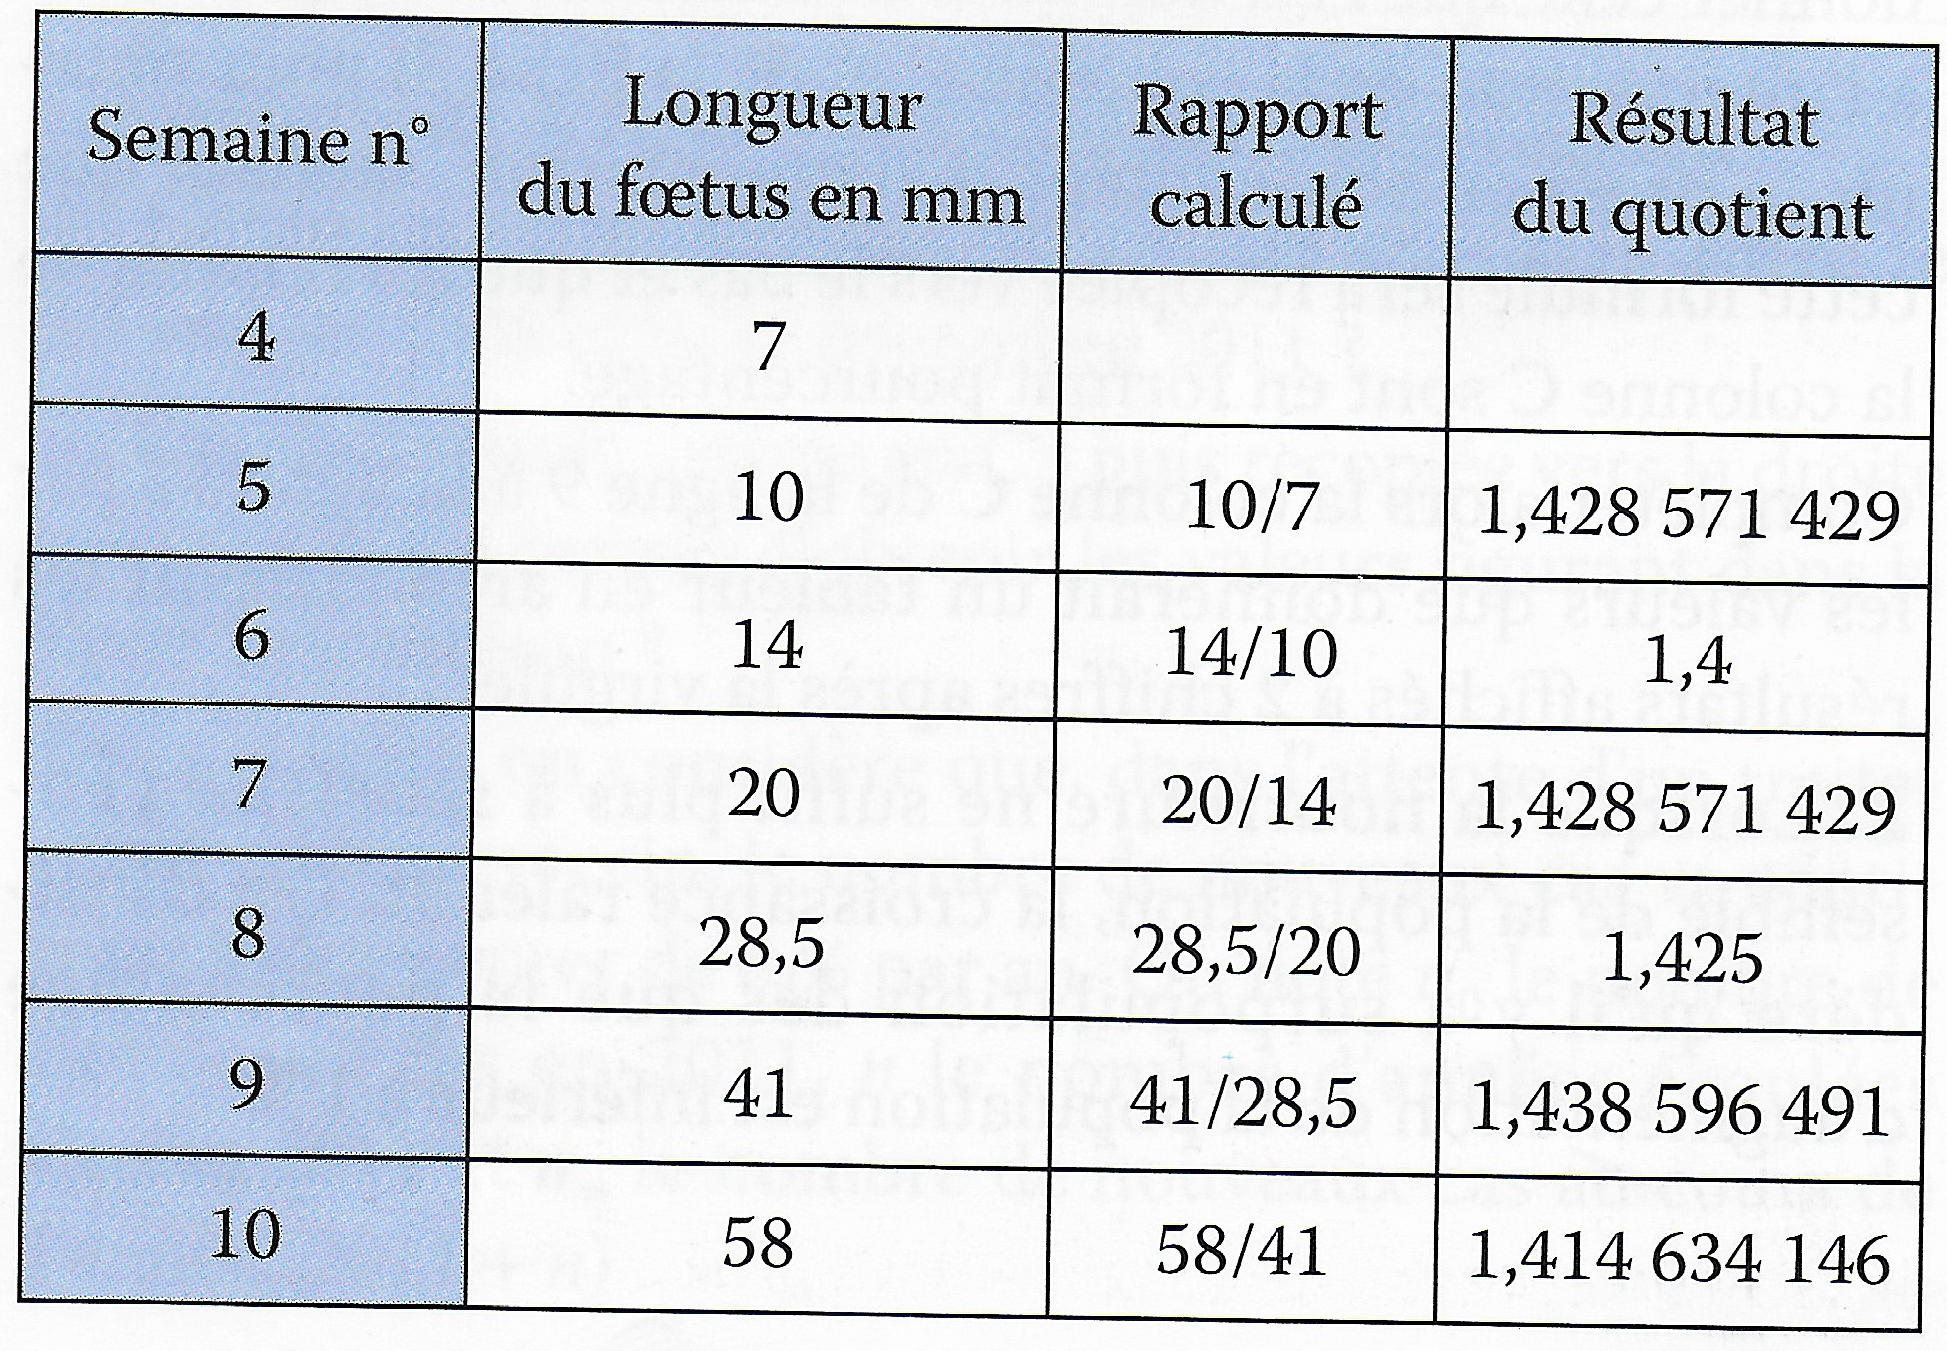
\includegraphics[scale=0.2]{tabl_foetus}
		\end{center}
		
		Pour simplifier, on retient \num{1.42} comme valeur approchée des résultats de la dernière colonne. Quelle est l'augmentation en pourcentage de la taille du f\oe tus en une semaine ?
		
		\begin{solution}
			\begin{equation*}
				\num{1.42} - 1 = \num{0.42}
			\end{equation*}
			
			Donc chaque semaine, la taille du f\oe tus augmente de 42 \%.
		\end{solution}
		
	\question[4]
		On considère la suite géométrique $(u_n)$ de raison \num{1.42} et telle que $u_0 = 7$. Le terme $u_n$ de rang $n$ représenterait la taille du f\oe tus en mm la semaine 4 + $n$.
		\begin{parts}
			\part[1] Que représenterait $u_{16}$ ?
				\begin{solution}
					$u_{16}$ représenterait la taille du f\oe tus en mm la semaine 20 (4 + 16).
				\end{solution}
			\part[1] Calculer une valeur approchée à l'unité de $u_{16}$.
				\begin{solution}
					\begin{eqnarray*}
						u_{16} & = & 7 \times \num{1.42}^{16} \\
						u_{16} & = & \num{1913}
					\end{eqnarray*}
				\end{solution}
			\part[2] Le modèle <<suite géométrique>> est-il pertinent au bout de 20 semaines ?
				\begin{solution}
					Si on suit ce modèle, à la vingtième semaine le f\oe tus mesurerait 1913 millimètres, soit presque 2 mètres. Ce n'est pas réaliste, donc le modèle n'est pas pertinent.
				\end{solution}
		\end{parts}
\end{questions}